\RequirePackage{fix-cm}
\documentclass[preprint,12pt, review]{elsarticle}
\usepackage[T1]{fontenc}

\usepackage{graphicx}
\usepackage{tkz-graph}
\usepackage{amsmath, amssymb}
\usepackage{amsthm}
\usepackage{multirow}
\usepackage{graphicx}
\usepackage{tikz}
\usepackage{amsfonts}
\usepackage{subcaption}
\usepackage{hyperref}

\usepackage{color}	% Different font colors
\usepackage{enumerate}
\usepackage{enumitem}
\usepackage{mathtools}
\usepackage{color}
\usepackage[linesnumbered]{algorithm2e}
\SetKwRepeat{Do}{do}{while}

\captionsetup{compatibility=false}

\newtheorem{theorem}{\textbf{Theorem}}
\newtheorem{observation}[theorem]{\textbf{Observation}}
\newtheorem{definition}{\textbf{Definition}}
\newtheorem{problem}{\textbf{Problem}}
\newtheorem{proposition}[theorem]{\textbf{Proposition}}
\newtheorem{remark}[theorem]{\textbf{Remark}}
\newtheorem{lemma}[theorem]{\textbf{Lemma}}

\tikzset{
every edge/.style={fill=none} 
every node/.style={shape=circle,fill=gray!40,draw }}

\journal{Discrete Applied Mathematics}
%
\begin{document}
\begin{frontmatter}

\title{Computing the broadcast time of a graph}

\author{Marika Ivanova\corref{cor1}}
\ead{Marika.Ivanova@uib.no}
\cortext[cor1]{Corresponding author}

\author{Dag Haugland\corref{cor2}}
\ead{Dag.Haugland@uib.no}

\address{Department of Informatics, University of Bergen, Norway}


\date{Received: date / Accepted: date}

\begin{abstract}
Given a graph and a subset of its nodes, referred to as source nodes, the minimum broadcast problem asks for the minimum number of steps in which a signal can be transmitted from the sources to all other nodes in the graph.
In each step, the sources and the nodes that already have received the signal can forward it to at most one of their neighbor nodes.
The problem has previously been proved to be NP-hard. 
In the current work, we develop a compact integer programming model for the problem.
We also devise procedures for computing lower bounds on the minimum number of steps required, along with methods for constructing near-optimal solutions.
Computational experiments demonstrate that in a wide range of instances, the lower and upper bounds under study collapse.
In instances where this is not the case, the integer programming model proves strong capabilities in closing the remaining gap.

\begin{keyword}
Graph \sep Communication \sep Integer Programming \sep Bounds
\end{keyword}
\end{abstract}
\end{frontmatter}

\section{Introduction}
\label{intro}
The minimum broadcast time (MBT) problem is identified by a graph and a subset of its nodes,
referred to as source nodes.
Each node in the graph corresponds to a communication unit.
The task is to disseminate a signal from the source nodes to all other nodes in a shortest possible time (broadcast time), while abiding by communication rules.
A node is said to be \emph{informed} at a given time if it is a source, or it already has received the signal from some other node.
Otherwise, the node is said to be \emph{uninformed}.
Consequently, the set of informed nodes is initially exactly the set of sources.
Reflecting the fact that communication can be established only between pairs of nodes that are located within a sufficiently close vicinity of each other,
the edge set of the graph consists of potential communication links along which the signal can be transmitted.

The time is divided into a finite number of steps.
Every informed node can, in each time step, forward the signal to at most one uninformed neighbor node.
Therefore, the number of informed nodes can at most be doubled from one step to the next.
This communication protocol appears in various practical application such as communication among computer processors or telephone networks.
Situations where the signals have to cover large distances typically assume sending the signal to one neighbor at the time.
Inter-satellite communication networks thus constitute a prominent application area \cite{chu17}.
In particular, the MBT problem arises when one or a few satellites need to broadcast data quickly by means of time-division multiplexing.

The current literature on MBT offers some theoretical results, including complexity and approximability theorems.
Although inexact solution methods also have been proposed, few attempts seem to be made in order to compute the exact optimum,
or to find lower bounds on the minimum broadcast time.
The goal of the current text is to fill this gap, and we make the following contributions in that direction:

First, a compact integer programming model is developed.
While the model targets the exact minimum in instances of moderate size, its continuous relaxation is suitable for computation of lower bounds in larger instances.
Second, we derive lower bounding techniques, both of an analytical nature and in terms of a combinatorial relaxation of MBT,
that do not rely on linear programming.
Third, we devise an upper bounding algorithm, which in combination with the lower bounds is able to close the optimality gap in a wide range of instances.

The remainder of the paper is organized as follows:
Next, we review the current scientific literature on MBT and related problems,
and in Section \ref{sec:def}, a concise problem definition is provided.
The integer program is formulated and discussed in Section \ref{sec:exact}.
Lower and upper bounding methods are derived in Section \ref{sec:lb} and \ref{sec:ub}, respectively.
Computational experiments are reported in Section \ref{sec:exp}, before the work is concluded by Section \ref{sec:conc}.

\subsection{Literature overview} \label{sec:litrev}

Deciding whether an instance of MBT has a solution with broadcast time at most $t$ has been shown to be NP-complete \cite{slater81}. 
For bipartite planar graphs with maximum degree 3, NP-completeness persists even if $t=2$ or if there is only one source \cite{jansen95}.
When $t=2$, the problem also remains NP-complete for cubic planar graphs \cite{middendorf93}, grid graphs with maximum degree 3,
complete grid graphs, chordal graphs, and for split graphs \cite{jansen95}. 
The single-source variant of the decision version of MBT is NP-complete for grid graphs with maximum degree 4, and for chordal graphs \cite{jansen95}.
The problem is known to be polynomial in trees \cite{slater81}.
Whether the problem is NP-complete for split graphs with a single source was stated as an open questions in \cite{jansen95}, and has to the best of our knowledge not been answered yet.

A number of inexact methods, for both general and special graph classes, have been proposed in the literature during the last three decades.
One of the first works of this category \cite{scheuermann84} 
introduces a dynamic programming algorithm based on generating all maximum matchings in an induced bipartite graph.
Additional contributions of \cite{scheuermann84} are heuristic approaches for near optimal broadcasting.
From more recent works we mention \cite{hasson04}, which describes a meta heuristic algorithm for MBT, and provides a comparison with other existing methods.
The communication model is considered in an existing satellite navigation system in \cite{chu17}, where a greedy inexact method is proposed together with a mathematical programming model.
Examples of additional efficient heuristics can be found e.g. in \cite{harutyunyan06,harutyunyan14,wang10,jimborean13}.

Approximation algorithms for MBT are studied in \cite{kortsarz95}. 
The authors argue that methods presented in \cite{scheuermann84} provide no guarantee on the performance, and show that a wheel-graph is an example of an unfavourable instance.
They introduce an $\mathcal{O}(\sqrt{n})$-additive approximation algorithm for broadcasting in general graphs with $n$ nodes.
They further provide approximation algorithms for several graph classes with small separators with approximation ratio proportional to the separator size times $\log n$.
Throughout the text, the symbol $\log$ refers to the logarithm of base 2.
Another algorithm with $\mathcal{O}\left(\frac{\log n}{\log \log n}\right)$-approximation ratio is given in~\cite{elkin03}.
Most of the works cited above consider a single source.

A related problem extensively studied in the literature is the minimum broadcast graph problem \cite{grigni91,mcgarvey16}. 
A broadcast graph supports a broadcast from any node to all other nodes in optimal time $\lceil\log n\rceil$.
For a given integer $n$, a variant of the problem is to find a broadcast graph of $n$ nodes such that the number of edges in the graph is minimized.
In another variant, the maximum node degree rather than the edge cardinality is subject to minimization.
MgGarvey et al.\ \cite{mcgarvey16} study integer linear programming (ILP) models for $c$-broadcast graphs, which is a generalization where signal transmission to at most $c$ neighbours is allowed in a single time step.

Despite a certain resemblance with MBT, the minimum broadcast graph problem is clearly distinguished from our problem,
and will consequently not be considered further in the current work.

\section{Network Model and Definitions} \label{sec:def}

The communication network is represented by a connected graph $G=(V,E)$ and a subset $S\subseteq V$ referred to as the set of sources.
We denote the number of nodes and the number of sources by $n=|V|$ and $\sigma=|S|$, respectively. 

\begin{definition} \label{def:broadcasttime}
The \emph{broadcast time} $\tau(G,S)$ of a node set $S\subseteq V$ in $G$ is defined as the smallest integer $t\geq 0$ for which there exist
a sequence $V_0\subseteq\dots\subseteq V_t$ of node sets and a function $\pi:V\setminus S\to V$, such that:
\begin{enumerate}
  \item $V_0=S$ and $V_t=V$, \label{def:boundary}
  \item for all $v\in V\setminus S$, $\{v,\pi(v)\}\in E$, \label{def:edge}
  \item for all $i=1,\ldots,t$ and all $v\in V_i$, $\pi(v)\in V_{i-1}$, and \label{def:parent}
  \item for all $u,v\in V_i\setminus V_{i-1}$, $\pi(u)=\pi(v)$ only if $u=v$. \label{def:unique}
\end{enumerate}
\end{definition}

Referring to Section \ref{intro}, the node set $V_i$ is the set of nodes that are informed in time step $i$.
Initially, only the sources are informed ($V_0=S$), whereas all nodes are informed after $t$ time steps ($V_t=V$),
and the set of informed nodes is monotonously non-decreasing ($V_{i-1}\subseteq V_i$ for $i=1,\ldots,t$).
The parent function $\pi$ maps each node to the node from which it received the signal.
Conditions \ref{def:edge}--\ref{def:parent} of Definition \ref{def:broadcasttime} thus reflect that the sender is a neighbor node in $G$,
and that it is informed at an earlier time step than the recipient node.
Because each node can send to at most one neighbor node in each time step,
condition \ref{def:unique} states that $\pi$ maps the set of nodes becoming informed in step $i$ to distinct parent nodes.

The optimization problem in question is formulated as follows:
\begin{problem}[\textsc{Minimum Broadcast Time}]\label{prob:min}
Given $G=(V,E)$ and $S\subseteq V$, find $\tau(G,S)$.
\end{problem}

\begin{definition} \label{def:broadcastgraph}
For any $V_0,\ldots,V_t$ and $\pi$ satisfying the conditions of Definition \ref{def:broadcasttime},
the corresponding \emph{communication forest} is
the digraph $D=(V,A)$, where $A=\left\{\left(v,\pi(v)\right): v\in V\right\}$.
Each connected component of $D$ is a \emph{communication tree}.
\end{definition}

\noindent
It is easily verified that the communication trees are indeed arborescences, rooted at distinct sources, with arcs pointing away from the source.
Let $T(s)=\left(V(s),A(s)\right)$ denote the communication tree in $D$ rooted at source $s\in S$,
and let $T_i(s)$ be the subtree of $T(s)$ induced by $V(s)\cap V_i$.
Analogously, let $D_i$ be the directed subgraph of $D$ induced by node set $V_i$.
For the sake of notational simplicity, the dependence on $(V_0,\ldots,V_t,\pi)$ is suppressed when referring to the directed graphs introduced here.

The degree of node $v$ in graph $G$ is denoted by $\delta_G(v)$.
The set of neighbors of $v\in V$ in $G$ is denoted by $N_G(v)$.
% Whenever there is no risk of confusion, the subscript $G$ is omitted.
For a given subset $U\subseteq V$ of nodes, we define $N_G(U)=\bigcup_{v\in U}N_G(v)$.

Likewise, $\delta^-_D(v)$ and $\delta^+_D(v)$ denote, respectively, the in-degree and the out-degree of $D$,
and $N_D^+(v)=\left\{u\in V:(v,u)\in A\right\}$ and $N_D^-(v)=\left\{u\in V:(u,v)\in A\right\}$ denote the neighbor sets of node $v$ in $D$.

\section{Exact methods}

Problem \ref{prob:min} can be formulated as an integer linear program. % and solved to optimality. 
In this section, we present two different modeling approaches. 

\subsection{Broadcast time model}
The first studied model is a straightforward formulation of the problem.
Consider variables 
$$ x_{uv}^k=
\begin{cases} 
1, \text{ if } v\in V_k \text{ and } \pi(v)=u,\\ 
0, \text{ otherwise},
\end{cases}
z_{k}=\begin{cases}
1, \text{ if } k\leq\tau(G,S),\\
0, \text{ otherwise}.
\end{cases}
$$
The worst case scenario is when $G$ is a path $v_1,\dots,v_n$ with $S=\{v_1\}$. 
In such an instance, the necessary number of time steps is $n-1$, which gives a trivial upper bound $\bar{t}=n-s$ on the broadcast time.
Problem \ref{prob:min} is then formulated as follows: 
\begin{subequations}\label{mod:basic}
\begin{align}
\label{mod:basic:obj} \min \sum\limits_{k=1}^{\bar{t}}z_k \\ 
\notag \text{s. t. } \\
\label{mod:basic:onefromroot} \sum_{v \in N(s)}x^1_{sv} & \leq 1 & s\in S,\\
\label{mod:basic:singlein} \sum\limits_{k=1}^{\bar{t}}\sum\limits_{v\in N(u)}x_{vu}^k & = 1 & u\in V \setminus S,\\
%\label{mod:basic:uniqueTout} \sum\limits_{v\in N(u)}x_{uv}^k & \leq 1  & u\in V,k=1,\dots,\bar{t},\\
\label{mod:basic:tIncreases} \sum\limits_{v\in N(u)}x_{uv}^k &\leq\sum\limits_{\ell=1}^{k-1}\sum\limits_{w\in N(u)} x_{wu}^{\ell}  & u\in V\setminus S, k=2,\dots,\bar{t},\\
%\label{mod:basic:tIncreases} x_{uv}^k &\leq\sum\limits_{\ell=1}^{k-1}\sum\limits_{w\in N(u)\setminus\{v\}} x_{wu}^{\ell}  & \{u,v\}\in E, u\not\in S, k=2,\dots,\bar{t},\\
%\label{mod:basic:tcrel} \sum\limits_{k=1}^{\bar{t}}k\cdot x_{uv}^k & \leq t^* &  (u,v)\in A,\\
\label{mod:basic:tcrel} \sum\limits_{v\in N(u)}x_{uv}^k & \leq z_k &  u\in V,k=1,\dots,\bar{t},\\
%\label{mod:basic:tcrel} \sum\limits_{t=1}^{n-1}t\sum\limits_{j\in N(i)}x_{ij}^k & \leq c &  i\in V,\\
\label{mod:basic:positiveCost}x_{uv}^1 & = 0 & (u,v)\in A, u \in V\setminus S,\\
\label{mod:basic:dim}&&x \in \{0,1\}^{A\times V},z\in\{0,1\}^{\bar{t}}.
\end{align}~
\end{subequations}
%Constraints \eqref{mod:basic:onefromroot} indicate that for each source node $s$, there is at most one adjacent node $u\in V_1$ such that $\pi(u)=s$.
Constraints \eqref{mod:basic:onefromroot} indicate that each source node $s$ forwards the signal to at most one adjacent node $v$ in the first time step. 
%By \eqref{mod:basic:singlein}, for every non-source node $u$, there is exactly one node $v$ such that $\pi(u)=v$.
By \eqref{mod:basic:singlein}, every non-source node $u$ receives the signal from exactly one adjacent node $v$ in some time step $k$.
%The requirement that a non-source node has a neighbor $v\in V_k$ such that $\pi(v)=u$ only if there exists a node $w\in V_{k-1}$ such that $\pi(u)=w$ is modeled by \eqref{mod:basic:tIncreases}. 
The requirement that a non-source node $u$ informs a neighbor $v$ in the $k$-th time step only if $u$ is informed by some adjacent node $w$ in an earlier time step is modeled by \eqref{mod:basic:tIncreases}. 
%Constraints \eqref{mod:basic:uniqueTout} enforce that for each node $u\in V$ and each subset $V_k$, there is at most one adjacent node $v\in V_k$ with $\pi(v)=u$.
Constraints \eqref{mod:basic:tcrel} enforce that each node $u\in V$ forwards the signal to at most one adjacent node $v$ in each time step.
It also sets a correct value to the variable $z$ that appears in the objective function.
%The requirement that only informed nodes can relay a signal is modeled by \eqref{mod:basic:tIncreases}. 
%The maximum time step at which any transmission takes place is captured by \eqref{mod:basic:tcrel}, and finally, \eqref{mod:basic:positiveCost} states that a node that is not a source never transmits in the first time step.
%The length of the sequence of subsets is captured by \eqref{mod:basic:tcrel}, and finally, \eqref{mod:basic:positiveCost} state that if $\pi(v)\not\in S$ for some $j\in V$, then $v\not\in V_1$.
Finally, \eqref{mod:basic:positiveCost} state that non-source nodes do not transmit in the first time step.

%In Model \ref{mod:basic}, superscript of $x$-variables represents a time step in which a signal is transmitted along corresponding arc.
\subsubsection{Decision version}
\label{sec:decbasic}
The nature of MBT suggests another modelling approach derived from Model \ref{mod:basic}. 
For a given maximum broadcast time $t_{\text{max}}$, we maximize the number of nodes $v$ that receive a signal from some neighbor $u$ within $t_{\text{max}}$ time steps.
If the optimal value is $n-s$, it is clear that we found a spanning broadcast tree with broadcast time $t_{\text{max}}$.
In case the optimal value is less than $n-s$, the given $t_{\text{max}}$ is insufficient, and we have to try solving the problem with increased time limit.
Clearly, an additional knowledge of upper and lower bound spares some computations. 
A lower bound is the initial value of $t_{\text{max}}$. 
Similarly, if an upper bound $\bar{t}$ is known and $t_{\text{max}}=\bar{t}-1$, the process can be terminated even when the objective function is less then $n-s$, because $\bar{t}$ is than the optimal value.

The decision model \ref{mod:basic:dec}  has the form
\begin{subequations}\label{mod:basic:dec}
\begin{align}
\label{mod:basic:dec:obj} \max \sum\limits_{v \in V\setminus S}\sum\limits_{u \in N(v)} \sum\limits_{k=1}^{t_{\text{max}}}x_{uv}^k \\ 
\notag \text{s. t. } \\
\label{mod:basic:dec:atMost1in} \sum\limits_{k=1}^{t_{\text{max}}}\sum\limits_{v\in N(u)}x_{vu}^k & \leq 1 & u\in V \setminus S,\\
\label{mod:basic:dec:0toSource} \sum\limits_{k=1}^{t_{\text{max}}}\sum\limits_{v\in N(u)}x_{vu}^k & = 0  & u\in S,\\
\notag \eqref{mod:basic:onefromroot}, \eqref{mod:basic:tIncreases}, \eqref{mod:basic:positiveCost},\\
\label{mod:basic:dec:dim}&&x \in \{0,1\}^{A\times V}.
\end{align}~
\end{subequations}

Constraint \eqref{mod:basic:singlein} is replaced by \eqref{mod:basic:dec:atMost1in} and \eqref{mod:basic:dec:0toSource}. 
The former is an inequality, because not all nodes are necessarily reached within the given time limit.
The latter makes sure that sources are not reached by any signal. 
This was filtered out by optimality in \eqref{mod:basic}, but it must be forbidden explicitly in \eqref{mod:basic:dec} due to the changed objective function.
The actual target function is the minimum time required for spreading the signal to all nodes, and so we are looking for the smallest value of $t_{\text{max}}$.
\subsection{Binomial tree model}

The binomial tree $B^k$ of order $k$ is an ordered tree defined recursively as follow \cite{cormen90}:
\begin{itemize}
\item The binomial tree $B^0$ consists of a single node.
\item The binomial tree $B^k$ has a root with $k$ children where the $i$-th child is the root of a binomial tree of order $k-i$, $i=1,\dots,k$.
\end{itemize}
An example of $B^3$ is depicted in Fig.\ref{fig:beta}.
%If a solution to MBT consists of broadcast trees that are binomial, the number of informed nodes doubles in each time step.
For a given time step $k$, the maximum number of informed nodes within $k$ steps is $|S|2^k$.
This occurs when the solution of MBT consists of broadcast trees that are binomial.
%Any broadcast tree can be regarded as pruned binomial tree.  
%Problem \ref{prob:min} can therefore be restated as finding a partition of $G$ into $m$ pruned binomial trees 
\begin{observation}
\label{obs:btspread}
if $r\in S$ is the root of $B^k$, then $\tau(B^k,\{r\})=k$.
\end{observation}
\begin{figure}
\centering
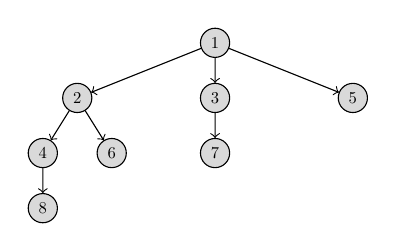
\begin{tikzpicture}[->,scale=.7,every node/.style = {scale=.6,draw,shape=circle, align=center, fill=gray!30}, level/.style={sibling distance=2.5cm/#1,level distance=1.0cm}]]
   \node[] {1}
   	   child[] { node {2} 
	   	   child {node {4}
		  	child {node {8}} 
		   }
		   child {node {6} }
	   }
   child[] { node {3}
   	   child { node {7} }
	   }
   child[] { node {5}
	}
 ;
\end{tikzpicture}
\caption{A binomial tree with nodes labeled by their positions}
\label{fig:beta}
\end{figure}

\subsubsection{Binomial trees over positive integers}

Let $k\in \mathbb{N}$ and $I=\{1,\dots,2^k\}$. 
A directed binomial tree $B^k=(V_{B^k},A_{B^k})$ with arcs oriented towards the leaves has a regular structure that allows to define a systematic numbering of nodes so that a node number determines unambiguously a position in $B^k$.
That is, we need an applicable bijective function $\beta:V_{B^k}\to I$.
A suitable bijection $\beta$ assigns values from $I$ to nodes increasingly with decreasing outgoing degree.
If there is an ambiguity, a node whose parent has a lower number is assigned a lower number.
This function is defined recursively as
\begin{equation*}
\label{eq:beta}
\beta(v)=\begin{cases}
1,\text{ if } v \text{ is the root of } B^k,\\
\beta(u) + 2^{k-deg^+(v)-1}, (u,v)\in A_{B^k},\text{ otherwise}.
\end{cases}
\end{equation*}
Nodes in Fig. \ref{fig:beta} are labeled with their $\beta$-values.
Pairs of integers that are assigned to adjacent nodes in a binomial tree are defined by relation
\begin{equation*}
\label{eq:betarel}
R=\{(i,j)\in\mathbb{N}\times\mathbb{N}:j=i+2^k,k\geq\log i,k\in \mathbb{Z}\}.
\end{equation*}

We further define the function $\pi':\mathbb{N}\to\mathbb{Z}_+$ that for a given integer $i$ associated with node $v$
determines $\beta$-value of parent of $v$: 
\begin{align*}
\label{eq:piprime}
\pi'(1)&=0,& \\
\pi'(j)&=j-2^{\lceil\log j\rceil -1}, &j > 1.
\end{align*}
Using functions $\alpha$, $\beta$, $\pi'$ and the relation $R$, we introduce the notion of binomial trees over positive integers.
\begin{definition}
A pair $(I,X)$ where $I=\{1,\dots,2^k\}$, $k\in\mathbb{Z}_+$, $(\alpha(u),\beta(u))=(\alpha(v),\beta(v))\Leftrightarrow u=v$ and
$X=\{(i,j)\in R, i,j\in I\}$ is an \emph{integer binomial tree of order $k$}. 

$(I,X)$, where $I\subseteq\{1,\dots,2^k\}, k\in \mathbb{Z}_+,\pi(j)\in I$ for all $j\in I\setminus\{1\}$ and
$X=\{(i,j)\in R, i,j\in I\}$ is an \emph{integer binomial tree of order $k$ pruned at $\{1,\dots,2^k\}\setminus I$}.
\end{definition}
We now develop a method for modelling Problem \ref{prob:min} whose main principle is finding a partition of $G$ into pruned binomial trees.
For any integer $i$, let $I_i=\{2^{i-1}+1,\dots,2^i\}$.
%\begin{problem}
%\label{prob:dec}
%Given $G=(V,E)$, $S\subseteq V$ and $t\in \mathbb{N}$, is there a sequence $S=V_0\subseteq\dots\subseteq V_t=V$ 
%and a mapping $\pi:V\setminus S\to V$, such that for each $v\in V\setminus S:\{v,\pi(v)\}\in E$ and for each  $u,v\in V_i\setminus V_{i-1}: \pi(u)\neq \pi(v)\Leftrightarrow u\neq v$?
%\end{problem}
%For a delay $t$, at most $s\cdot 2^t$ nodes can be informed within $t$ steps. 
%Therefore, we assume $n\leq 2^ks.
%This can be achieved when the broadcast forest $T$ consists of binomial trees $B^t$ of order $t$ rooted at sources $s\in S$.
%Hence, if there is a partition of $G$ into $s$ pruned binomial trees of order at most $t$ rooted at sources, then $(G,S,t)$ is a YES instance of Problem \ref{prob:dec}.
%Finding a partition of $G$ into $s$ pruned binomial trees can be equivalently formulated as finding a partition of $G''$ into $s$ (complete) binomial trees, 
%where $G''$ is constructed from $G$ as follows:
%Let $\alpha\coloneqq s\cdot 2^k-|V|$, and let $K_\alpha=(V_\alpha,E_\alpha)$ be a complete graph on $\alpha$ nodes.
%Each node in $K_\alpha$ is connected to every node $v\in V$ in the original graph $G$.
%Thus, $G''=(V'',E'')$ with $V''=V\cup V_\alpha$ and $E''=E\cup E_\alpha\cup \{\{u,v\}: u\in V \wedge v\in V_\alpha\}$.
%The set of arcs $A''$ is constructed by creating two arcs of opposite orientation for each edge, but arcs with orientation from $V_\alpha$ to $V$ are excluded. 
%Formally, $A''=A\cup\{(u,v),(v,u): \{u,v\}\in E_\alpha\}\cup\{(u,v):u\in V \wedge v\in V_\alpha\}$.

%\begin{observation}\label{obs:deg}
%For each $i\in\{1,\dots,t\}$, the set $\{v\in V^t: 1\leq\beta(v)\leq2^i\}\setminus\{v\in V^t:1\leq\beta(v)\leq2^{i-1}\}$ contains nodes with out-degree $t-i$.
%\end{observation}
%\begin{observation}\label{obs:childdeg}
%Children of $v\in V^t$ with $\text{deg}^+(v)=\ell$ have out-degree $0,\dots,\ell-1$.
%\end{observation}
\begin{observation}\label{obs:eqbetalevel}
$\pi'$ is injective.
%For $i_1,i_2\in I_i$, $\pi'(i_1)=\pi'(i_2)\Leftrightarrow i_1=i_2$.
\end{observation}
\begin{proof}
We notice that $\lceil\log (2^{i-1}+1)\rceil=\dots =\lceil\log 2^i\rceil$, and thus $\pi'(2^{i-1}+1),\dots,\pi'(2^i)$ are pairwise different.\qed 
\end{proof}

\begin{proposition}\label{lem:probeq}
A graph $G=(V,E)$ and $S\subseteq V$ has $\tau(G,S)\leq k$ iff it is possible to assign integers to nodes
such that they form $m$ (pruned) integer binomial trees of order $k$ or smaller rooted at sources.
\end{proposition}
\begin{proof}
Assume nodes in $V$ can be labeled by integers from $I=\{1,\dots,2^k\}$ so that they form (pruned) integer integer binomial trees $B_\ell$ of order at most $k$, $1\leq\ell\leq m$.
For $r\in V_{B_\ell}$ with $\alpha(r)=r$ and $\beta(r)=1$, by Obs. \ref{obs:btspread}, $\tau(B_\ell,\{r\})\leq k$.
The sequence of node sets $V_0,\dots,V_k$ is constructed by setting $V_0=\{v\in V:\beta(v)=1\}$, and $V_{i}=V_{i-1}\cup\{v\in V: \beta(v)\in I_i\}$.
Moreover, $\pi(v)=u\Leftrightarrow \alpha(v)=\alpha(u)~\&~\pi'(\beta(v))=\beta(u)$.
Also, $\pi(u)=\pi(v)\Leftrightarrow u=v$ follows from Obs. \ref{obs:eqbetalevel}, because nodes in $V_i$ have $\beta$ values in $I_i$.

Conversely, suppose there is a sequence of subsets and a function $\pi$ in $G$ with the desired properties.
Nodes are associated with integers from $I$ assigned according to the following steps:
\begin{enumerate}
\item $\beta(s)=1$ for all $s\in V_0$,
\item For $v\in V_i$, set $\beta(v)=j$ such that $j\in I_i$ and $(\pi'(\beta(v)),j)\in R, 1\leq i\leq k$.  
\end{enumerate}
\qed
\end{proof}
\subsubsection{The formulation}
Consider a graph $G'=(V',E')$ constructed  by adding a universal node $v_0$ to $G$. 
The set of nodes and edges is then $V'=V\cup \{v_0\}$ and $E'=E\cup\{\{v_0,v\}:v\in V\}$.
Apart from $z$-variables introduced in model \eqref{mod:basic}, the ILP formulation based on partition into binomial trees uses 
$$
y_{is}^v=\begin{cases}
1, \text{ if } \beta(v)=i \text{ and } \alpha(v)=s,\\ 
0, \text{ otherwise},\\
\end{cases}
$$
where $v\in V'$, $i\in I$, $s\in S$ and $0\leq j\leq \bar{t}$. 
With the definition of $G'$ above, it is straightforward to specify constraints that enforce desired values for $y$-variables.
Whenever $y_{is}^{v_0}=1$, it indicates that the binomial tree rooted at $s$ is pruned at node with position $i$.
%An obvious weakness of this approach is  that the number of nodes increases to $|V''|=\mathcal{O}(ns)$, and the dimension of variables is thus $\mathcal{O}(n^2s^2)$.
%However, once a suitable partition is found, the arcs of binomial trees contained in $K_\alpha$ can be diversely shuffled while preserving the layour of binomial trees in $G$.
%Instead of adding the entire complete graph $K_\alpha$, a single node $v_0$ with a loop $(v_0,v_0)$ is connected as an apex to the original $G$.
%Let us denote this multigraph as $G'=(V',E')$, where $V'=V\cup\{v_0\}$, $E'=E\cup\{\{u,v_0\}:u\in V\}\cup\{\{v_0\}\}$. 
%The arc set is then analogously defined as $A'=A\cup\{(u,v_0): u\in V\}\cup\{(v_0,v_0)\}$.
%The requirement for partition into binomial trees has to be adjusted accordingly.
%The subtrees contained in $G$ remain unchanged, every arc $(u,v)\in A^k_i, i=1,\dots,s$ in $G''$ with $u\in V$ and $v\in V_\alpha$ becomes $(u,v_0)$ in $G'$,
%and every $(u,v)\in A_\alpha$ becomes $(v_0,v_0)$.
%So, $v_0$ acts as a universal node that can substitute several nodes in each binomial tree.
Let us define the set $C(i)$ of $\beta$-positions of children (direct descendants) of node $v$ with $\beta(v)=i$ in a binomial tree of order $k$:
\begin{equation}
\label{eq:c1}
C(i)=\{2^j+i:j=\lceil\log_2 i\rceil,\dots,k-1\}.
\end{equation}
The formulation based on binomial trees is the following:
\begin{subequations}\label{mod:partition}
\begin{align}
\notag &\min\sum\limits_{j=0}^{\bar{t}}z_j,\\
\notag \text{s. t. } \\
\label{mod:part:nodeBelongs} \sum\limits_{i\in I}\sum\limits_{s\in S}y^v_{is} & = 1 & v\in V,\\
\label{mod:part:treeHasIJ} \sum\limits_{v\in V'}y^v_{is} & = 1 & i\in I,s\in S,\\
\label{mod:part:source1} y_{1s}^s & = 1  & s\in S,\\
%\label{mod:part:noReturn} y^u_{ij}+y^v_{lj} &\leq 1 & i\in I,l\in C(i), j\in J, u\in V_\alpha,v\in V,\\
%\label{mod:part:followArcs} y^u_{is}+y^v_{\ell s} &\leq 1 & i\in I,\ell\in C(i), s\in S, u,v\in V',(u,v)\not\in A',\\
%\label{mod:part:followArcsA} y^u_{is}+y^v_{\ell s} &\leq 1 & i\in I,\ell\in C(i), s\in S, u,v\in V,\{u,v\}\not\in E,\\
%\label{mod:part:followArcsB} y^{v_0}_{is}+y^v_{\ell s} &\leq 1 & i\in I,\ell\in C(i), s\in S, v\in V,\\
%\label{mod:part:followArcsA}y^{v_0}_{is}+y^u_{i s} + \sum\limits_{v\in V\setminus N(u)}y^v_{\ell s}&\leq 1 & u\in V,i\in I,\ell\in C(i), s\in S,  \\
%\label{mod:part:followArcsB}y^{v_0}_{is}+y^u_{\ell s} + \sum\limits_{v\in V\setminus N(u)}y^v_{i s}&\leq 1 & u\in V,i\in I,\ell\in C(i), s\in S,\\ 
\label{mod:part:followArcsA}\sum\limits_{v\in \bar{N}(u)}y^v_{\ell s}&\leq \sum\limits_{v\in N(\bar{N}(u))}y_{is}^{v} & u\in V,i\in I,\ell\in C(i), s\in S,  \\
\label{mod:part:followArcsB}\sum\limits_{v\in \bar{N}(\bar{N}(u))}y^v_{\ell s}&\leq \sum\limits_{v\in N(u)} y_{is}^{v} & u\in V,i\in I,\ell\in C(i), s\in S,\\ 
\label{mod:part:yzrel}\sum\limits_{v\in V}y^v_{is} & \leq z_{\lceil\log i\rceil} & i\in I,s\in S,\\
\label{mod:part:dim}&&y \in \{0,1\}^{I\times S\times V'}, z\in \{0,1\}^{\bar{t}}.
\end{align}~
\end{subequations}

%As the model represents the decision problem, it suffices to find any feasible solution, and no objective function is needed.
The interpretation of constraints \eqref{mod:part:nodeBelongs} is that every node in the original graph $G$ belongs to exactly one binomial tree.
Note that these constraints are quantified only over $V$ and not over $V'$.
In this way it is achieved that $v_0$ can be regarded as a part of several binomial trees.
By \eqref{mod:part:treeHasIJ} is ensured that exactly one node, possibly $v_0$, is allocated to position $i$ of each binomial tree.
By the summation over $V'$ is ensured, that pruned nodes are collectively represented by $v_0$.
Next, \eqref{mod:part:source1} enforce that source nodes are always the first nodes in corresponding binomial trees, in accordance with definition \eqref{eq:beta} of the function $\beta$.
The remaining two sets of constraints guarantee that the arcs of binomial trees follow edges in $E$.
%In particular, it is enforced by \eqref{mod:part:followArcsA} that if $u$ and $v$ are not adjacent in $G$, then $v$ must not act as a child of $u$ in any binomial tree.
In particular, it is enforced by \eqref{mod:part:followArcsA} that if there is some  non-neighbor $v$ of $u$  with a label $\ell$ in a binomial tree rooted at $s$,
then there must be a neighbor of some non-neighbor of $u$ with label $i$ in the same binomial tree.
Similarly, Constraints \eqref{mod:part:followArcsB} state that if there is a node $v$ with label $\ell$ in a binomial tree rooted at $s$ in the complement of neighborhood of all non-neighbors of $u$,
there must also be a neighbor of $u$ with label $i$ in this binomial tree. 
This reflects the obvious fact that if a tree is pruned at some node, all its descendants must also be excluded from the tree.
%The definition of $A'$ also prevents arcs of the binomial trees to be oriented from $V_\alpha$ to $V$.
%In other words, once the signal leaves the original graph $G$ and enters $v_0$, it cannot return back to $G$.
Without \eqref{mod:part:followArcsA} and \eqref{mod:part:followArcsB}, it could be possible to find a feasible solution, even when no partition of $G$ into pruned binomial trees exists.
Finally, the relation \eqref{mod:part:yzrel} between $y$ and $z$ variables follows from Obs. \ref{obs:btspread}. 
It says that whenever there is a node in a position $i$, then the delay is at least $\lceil\log i\rceil$.
%Constraints \eqref{mod:part:followArcsA} and \eqref{mod:part:followArcsB} can be replaced by stronger
%\begin{subequations}
%\begin{align}
%\label{mod:part:followArcsAStrongerA}
%y^{v_0}_{is}+y^u_{i s} + \sum\limits_{v\in V\setminus N(u)}y^v_{\ell s}&\leq 1 & u\in V,i\in I,\ell\in C(i), s\in S,  \\
%\label{mod:part:followArcsAStrongerB}
%y^{v_0}_{is}+y^u_{\ell s} + \sum\limits_{v\in V\setminus N(u)}y^v_{i s}&\leq 1 & u\in V,i\in I,\ell\in C(i), s\in S. 
%\end{align}
%\end{subequations}
%
\subsubsection{Valid inequalities}
Let $W$ be a maximal independent set in $G$.
Model \eqref{mod:partition} is strengthened by 
\begin{align}
\label{mod:part:vibasic}
y^{v_0}_{is}+ \sum\limits_{v\in W}(y^v_{is}+y^v_{\ell s})&\leq 1 & i\in I,\ell\in C(i), s\in S, 
\end{align}
which exploits the fact that no pair of nodes in $W$ is adjacent, and so there must be no two nodes with adjacent $\beta$-positions.

We now generalize this idea by using the notion of graph power $G^m=(V,E^m)$ commonly defined as a graph with the same set of nodes as $G$,
and an edge between two nodes in $G^m$ is present iff there is a path of length at most $m$ between them in $G$.
For our purposes, we use a slightly modified definition of the edge set
$$E^m=\{\{u,v\}:\text{there exists a path between $u$ and $v$ in $G$ of length $m$}\}.$$
Definition \eqref{eq:c1} can be generalized to descendants of an arbitrary distance $m$ from $v$ in $B^k$:
\begin{equation}
C^{m+1}(i)=\bigcup_{j\in C^1(i)}C^m(j).
\end{equation}
For a given $m$, let $W_m$ be a maximal independent set in $G^m$.
Further strengthening of model \eqref{mod:partition} is achieved by introducing valid inequalities
\begin{align}
\label{mod:part:vigeneral}
y^{v_0}_{is}+ \sum\limits_{v\in W_m}(y^v_{is}+y^v_{\ell s})&\leq 1 & i\in I,\ell\in C^m(i), s\in S,1\leq m\leq \Delta_G-1. 
\end{align}
Clearly, inequality \eqref{mod:part:vibasic} is included in \eqref{mod:part:vigeneral} for $m=1$.
The distance between positions $i$ and $\ell=C^m(i)$ in a binomial tree is $m$.
The maximal independent set $W_m$ contains nodes such that length of any path between any two nodes is different from $m$, 
and so there must not be two nodes in $W_m$ with positions $i$ and $\ell$ at the same time.

\subsubsection{Symmetry removal}
Another improvement of this model is achieved by a symmetry removal.
If a broadcast tree is identical to a binomial tree, we notice that nodes with labels from $C(i)$, i.e., children of some node $v$ with $\beta(v)=i$, are informed in increasing time steps.
For example in $B^3$, $C(2)=\{4,6\}$ and the corresponding nodes are informed in time step 2 and 3, respectively.
If a label $\ell\in C(i)$ corresponds to a node of a binomial tree that is pruned (if $y^{v_0}_{\ell s}=1$ for some $s\in S$), 
all labels $j\in C(i)$ such that $j>\ell$ can also be pruned. 
Thus, adding 
\begin{align}
\label{mod:part:sr}
y^{v_0}_{js}&\leq y^{v_0}_{\ell s}&i\in I,j,\ell\in C(i),j<\ell, s\in S
\end{align}
to the model reduces the set of feasible solutions.

\subsubsection{Decision version}

In a similar manner as we derived the decision version \eqref{mod:basic:dec} of model \eqref{mod:basic}, it is possible to construct a decision version of the binomial tree model \eqref{mod:partition} as follows:
\begin{subequations}\label{mod:genmatch}
\begin{align}
\notag \max\sum\limits_{v\in V}&\sum\limits_{i\in I}\sum\limits_{s\in S}   y_{is}^v,\\
\notag \text{s. t. } \\
\label{mod:genmatch:nodeBelongs} \sum\limits_{i\in I}\sum\limits_{s\in S}y^v_{is} & \leq 1 & v\in V,\\
\notag\eqref{mod:part:treeHasIJ} - \eqref{mod:part:followArcsB},\\
%\label{mod:genmatch:treeHasIJ} \sum\limits_{v\in V'}y^v_{is} & = 1 & i\in I,s\in V_T,\\
%\label{mod:genmatch:source1} y_{1s}^s & = 1  & s\in V_T,\\
%\label{mod:part:noReturn} y^u_{ij}+y^v_{lj} &\leq 1 & i\in I,l\in C(i), j\in J, u\in V_\alpha,v\in V,\\
%\label{mod:part:followArcs} y^u_{is}+y^v_{\ell s} &\leq 1 & i\in I,\ell\in C(i), s\in S, u,v\in V',(u,v)\not\in A',\\
%\label{mod:part:followArcsA} y^u_{is}+y^v_{\ell s} &\leq 1 & i\in I,\ell\in C(i), s\in S, u,v\in V,\{u,v\}\not\in E,\\
%\label{mod:part:followArcsB} y^{v_0}_{is}+y^v_{\ell s} &\leq 1 & i\in I,\ell\in C(i), s\in S, v\in V,\\
%\label{mod:genmatch:followArcsA}y^{v_0}_{is}+y^u_{i s} + \sum\limits_{v\in V\setminus N(u)}y^v_{\ell s}&\leq 1 & u\in V,i\in I,\ell\in C(i), s\in V_T,  \\
%\label{mod:genmatch:followArcsB}y^{v_0}_{is}+y^u_{\ell s} + \sum\limits_{v\in V\setminus N(u)}y^v_{i s}&\leq 1 & u\in V,i\in I,\ell\in C(i), s\in V_T,\\ 
\label{mod:genmatch:dim}&&y \in \{0,1\}^{I\times S\times V'}.
\end{align}~
\end{subequations}
This model is a modification of formulation \eqref{mod:partition}, and uses the same type of variables.
The objective function is to maximize the number of nodes involved in the binomial trees.
In order to determine the minimum broadcast time, we are looking for the minimum $k$ such that each node can be assigned a label from the set $I=\{1,\dots,2^k\}$ while satisfying given constraints.
%The index set $I=\{1,\dots,2^k\}$ depends on the input parameter $k$.
The constraints \eqref{mod:genmatch:nodeBelongs} state that each node belongs to at most one binomial tree.
Compared to \eqref{mod:part:nodeBelongs}, \eqref{mod:genmatch:nodeBelongs} is an inequality, because the binomial trees do not necessarily form a partition of $G$, and so not all nodes have to be used.
The remaining constraints are taken from formulation \eqref{mod:partition}. 

The approach is then analogous to the idea indicated in Section \ref{sec:decbasic}.
Assume we are given a lower bound $\underline{t}$ and an upper bound $\bar{t}$ on the minimum broadcast time.
Initially, we define the set $I=\{1,\dots,2^{\underline{t}}\}$ and iteratively solve the model while doubling the set $I$ until the objective function attains the value $n$.
That indicates that it is the first iteration in which all nodes are assigned a label, and it can be concluded that the minimum broadcast time is $\log_2|I|$.

%An objective function is naturally lacking in the formulation of the decision problem.
%It is nevertheless straightforward to create an ILP model for the corresponding optimization problem.
%Let $z_i=1 \Leftrightarrow t=i$ be a new variable and let $\bar{t}$ be an upper bound on the delay in $(G,S)$.
%Problem \ref{prob:min} is formulated as follows:
%\begin{subequations}
%\begin{align}
%\notag &\min\sum\limits_{j=0}^{\bar{t}}z_j,\\
%\notag \text{s. t. } \\
%\notag \eqref{mod:part:nodeBelongs} - \eqref{mod:part:source1},& \eqref{mod:part:followArcsAStrongerA} - \eqref{mod:part:followArcsAStrongerB}, \eqref{mod:part:vi}, \eqref{mod:part:sr},\\
%\notag\sum\limits_{v\in V}y^v_{is} & \leq z_{\lceil\log i\rceil} & i\in I,s\in S,\\
%\notag\label{mod:part:optdim}y &\in \{0,1\}^{I\times S\times V'}, z \in \{0,1\}^{\bar{t}}.
%\end{align}~
%\end{subequations}

\section{Lower bounds} \label{sec:lb}
Strong lower bounds on the minimum objective function value are of vital importance to combinatorial optimization algorithms.
In this section, we study three types of lower bounds on the broadcast time $\tau(G,S)$.

\subsection{Analytical lower bounds} \label{sec:lbanalyt}
Any solution $\left(V_0,\ldots,V_t,\pi\right)$ satisfying conditions \ref{def:boundary}--\ref{def:unique} of Definition \ref{def:broadcasttime},
also satisfies $\left|V_{k+1}\right|\leq 2\left|V_k\right|$ for all $k\geq 0$.
Combined with the observation made in Section \ref{sec:decbasic}, this yields the following bounds:
\begin{observation}
For all instances $(G,S)$ of Problem \ref{prob:min},
\begin{equation}
\left\lceil\log\frac{n}{\sigma}\right\rceil\leq \tau(G,S) \leq n-\sigma.
\label{eq:loglb}
\end{equation}
\label{obs:loglb}
\end{observation}

Consider the $m$-step Fibonacci numbers $\left\{f^{m}_k\right\}_{k=1,2,\ldots}$ \cite{noe05}, a generalization of the well-known (2-step) Fibonacci numbers, defined by
$f^{m}_k=0$ for $k\leq 0$, $f^{m}_1=1$, and 
other terms according to the linear recurrence relation 
\begin{align*}
f^{m}_k &=\sum\limits_{j=1}^m f^{m}_{k-j}, &\text{ for } k\geq 2.
\end{align*}

The generalized Fibonacci numbers are instrumental in the derivation of a lower bound on $\tau(G,S)$,
depending on the maximum node degree $d=\max\left\{\delta_G(v): v\in V\right\}$ in $G$.
The idea behind the bound is that the broadcast time can be no shorter than what is achieved if
the following ideal, but not necessarily feasible, criteria are met:
Every source transmits the signal to a neighbor node in each of the periods $1,\ldots,d$,
and every node $u\in V\setminus S$
transmits the signal to a neighbor node in each of the first $d-1$ periods following the period when $u$ gets informed.
An exception possibly occurs in the last period, as there may be fewer nodes left to be informed than there are nodes available to inform them.

\begin{proposition}
\begin{equation*}
\label{lem:lbreg1}
	\tau(G,S)\geq\min\left\{t:2\sigma\sum\limits_{j=1}^tf^{d-1}_j\geq n\right\}.
\end{equation*}
\label{prop:lbfib}
\end{proposition}
\begin{proof}

Consider a solution $\left(V_0,\ldots,V_t,\pi\right)$ with associated broadcast graph $D$, such that $V_{t-1}\neq V_t$, 
\begin{itemize}
  \item conditions \ref{def:boundary} and \ref{def:parent}--\ref{def:unique} of Definition \ref{def:broadcasttime} are satisfied,
  \item for each source $u\in S$ and each $j=1,\ldots,\min\{d,t-1\}$, there exists a node $v\in V_j\setminus V_{j-1}$ such that $\pi(v)=u$, and
  \item for each $k\in\{1,\ldots,t-2\}$, each node $u\in V_k\setminus V_{k-1}$, and each $j=k+1,\ldots,\min\{k+d-1,t-1\}$,
        there exists a node $v\in V_j\setminus V_{j-1}$ such that $\pi(v)=u$.
\end{itemize}
\noindent
Clearly, such a solution exists, and $\left(V_0,\ldots,V_t,\pi\right)$ is optimal if $\pi$ also satisfies condition \ref{def:edge} of Definition \ref{def:broadcasttime}.
We thus have $t\leq\tau(G,S)$.
It remains to prove that $2\sigma\sum_{k=1}^{t-1}f_k^{d-1}<n\leq 2\sigma\sum_{k=1}^tf_k^{d-1}$.

For $k=1,\ldots,t$, let $L_k=\left\{v\in V_k:\delta_{D_k}(v)=1\right\}$ denote the set of nodes with exactly one out- or in-neighbor in $D_k$,
and let $L_k=\emptyset$ for $k\leq 0$.
That is, for $i>1$, $L_k$ is the set of nodes that receive the signal in period $i$, whereas $L_1$ consists of all nodes informed in period 1, including the sources $S$.
Hence, $L_1,\ldots,L_{t-1}$ are disjoint sets (but $L_t$ may intersect $L_{t-1}$), and $V_k=L_1\cup\cdots\cup L_k$ for all $k=1,\ldots,t$.

Consider a period $k\in\{2,\ldots,t-1\}$.
The assumptions on $\left(V_0,\ldots,V_t,\pi\right)$ imply that $\pi$ is a bijection from $L_k$ to $L_{k-1}\cup\cdots\cup L_{k-d+1}$.
Thus, $\left|L_k\right|=\sum_{j=1}^{d-1}\left|L_{k-j}\right|$.
Since also $\left|L_1\right|=2\sigma=2\sigma f_1^{d-1}$ and $\left|L_j\right|=f_j^{d-1}=0$ for $j\leq 0$,
we get $\left|L_k\right|=2\sigma f_k^{d-1}$.
Further, $\left|L_t\right|\leq\sum_{j=1}^{d-1}\left|L_{t-j}\right|=2\sigma f_t^{d-1}$.
It follows that $2\sigma\sum_{k=1}^{t-1}f_k^{d-1}=\sum_{k=1}^{t-1}\left|L_k\right|=\left|V_{t-1}\right|<n=\left|V_t\right|\leq\sum_{k=1}^t\left|L_k\right|\leq 2\sigma\sum_{k=1}^tf_k^{d-1}$,
which completes the proof.
\end{proof}

\subsection{Continuous relaxations of integer programming models} \label{sec:lblprel}

For $t\in\mathbb{Z}_+$, define $\Omega(t)\subseteq[0,1]^{\overrightarrow{E}\times\{1,\ldots,t\}}$ as the set of feasible solutions to the continuous relaxation of
\eqref{mod:basic:dec:obj}--\eqref{mod:basic:dec:dim},
and let
\[
 \Omega^=(t) = \left\{x\in\Omega(t): \sum\limits_{u \in N(v)} \sum\limits_{k=1}^tx_{uv}^k = 1 ~~(v\in V\setminus S)\right\}.
\]
Let $t^{\ast}=\min\left\{t\in\mathbb{Z}_+: \Omega^=\neq\emptyset\right\}$ be the smallest value of $t$ for which the optimal objective function value in
the relaxation equals $n-\sigma$.
Existence of $t^{\ast}$ follows directly from $\Omega^=\left(\tau(G,S)\right)\neq\emptyset$.

% Consider a modification of model \eqref{mod:basic:dec:obj}--\eqref{mod:basic:dec:dim} where the coverage constraint
% $\sum\limits_{u \in N(v)} \sum\limits_{k=1}^tx_{uv}^k = 1$ is imposed on all non-source nodes $v\in V\setminus S$, and the objective is to minimize the communication time.
The continuous relaxation of \eqref{mod:basic:obj}--\eqref{mod:basic:dim} is feasible for sufficiently large $t$.
We denote its optimal objective function value by $\zeta(t)$.
% $\zeta(t)=\min\left\{\sum\limits_{k=1}^tz_k: x\in\Omega^=(t), z_k\geq\sum\limits_{u \in N(v)}x_{uv}^k ~~(k=1,\ldots,t, v\in V\setminus S)\right\}$.

\begin{proposition} \label{prop:lpweak}
For all $t\in\mathbb{Z}_+$ such that $\Omega^=(t)\neq\emptyset$, $\zeta(t)\leq t^{\ast}\leq\tau(G,S)$.
\end{proposition}
\begin{proof}
We first prove that $\zeta(t)$ is non-increasing with increasing $t$:
Let $\Gamma(t)$ denote the set of feasible solutions to the continuous relaxation of \eqref{mod:basic:obj}--\eqref{mod:basic:dim}, and assume $(x,z)\in\Gamma(t)$.
Define $\hat{x}\in[0,1]^{\overrightarrow{E}\times\{1,\ldots,t+1\}}$ such that
for all $(u,v)\in \overrightarrow{E}$, $\hat{x}_{uv}^k=x_{uv}^k$ ($k\leq t$) and $\hat{x}_{uv}^{t+1}=0$.
An analogous extension of $z$ to $\hat{z}\in[0,1]^{\{1,\ldots,t+1\}}$ yields $(\hat{x},\hat{z})\in\Gamma(t+1)$,
and $\sum_{k=1}^{t+1}\hat{z}_k=\sum_{k=1}^tz_k$ proves that $\zeta(t+1)\leq\zeta(t)$.

For $t\in\mathbb{Z}_+$ such that $\Omega^=(t)\neq\emptyset$, $t\geq t^{\ast}$ thus implies $\zeta(t)\leq\zeta(t^{\ast})$.
Since the only lower bounds on $z_k$ in \eqref{mod:basic:obj}--\eqref{mod:basic:dim} are $\max_{v\in V\setminus S}\sum\limits_{u \in N(v)}x_{uv}^k\leq 1$ and $z_{k-1}\leq 1$,
we get $\zeta(t)\leq\zeta(t^{\ast})\leq t^{\ast}$.
The proof is complete by observing that $t^{\ast}\leq\tau(G,S)$ follows from $\Omega^=\left(\tau(G,S)\right)\neq\emptyset$.
\end{proof}

\begin{remark} \label{rem:lpweak}
To compute a lower bound on $\tau(G,S)$, Proposition \ref{prop:lpweak} suggests to solve a sequence of instances of the continuous relaxation of problem \eqref{mod:basic:dec:obj}--\eqref{mod:basic:dec:dim},
and stop by the first value of $t$ for which the optimal objective function value is $n-\sigma$.
Such an approach yields a lower bound ($t^{\ast}$) on $\tau(G,S)$,
which is no weaker than the bound achieved by solving the continuous relaxation of \eqref{mod:basic:obj}--\eqref{mod:basic:dim}.
\end{remark}

\begin{remark} \label{rem:otheropt}
Remark \ref{rem:lpweak} applies to a reformulation of \eqref{mod:basic:obj}--\eqref{mod:basic:dim}, where a unique integer variable $y$ replaces $z_1,\ldots,z_t$,
and the objective is to minimize $y$ subject to the constraints
$y\geq\sum\limits_{k=1}^tk\sum\limits_{u \in N(v)}x_{uv}^k ~~(v\in V\setminus S)$, \eqref{mod:basic:singlein}--\eqref{mod:basic:tIncreases},
and \eqref{mod:basic:positiveCost}--\eqref{mod:basic:dim}.
\end{remark}

\subsection{Combinatorial relaxations} \label{sec:lbcombrel}

Lower bounds on the broadcast time $\tau(G,S)$ are obtained by omitting one or more of the conditions imposed in Definition \ref{def:broadcasttime}.
For the purpose of strongest possible bounds, the relaxations thus constructed can be supplied with conditions that are redundant in the problem definition.

Recall from Section \ref{sec:def} that $D=(V,A)$ denotes the communication forest corresponding to $\left(V_0,\ldots,V_t,\pi\right)$.
Conditions \ref{def:boundary}--\ref{def:unique} of Definition \ref{def:broadcasttime} imply that
\begin{enumerate}
\setcounter{enumi}{4}
  \item for all $v\in V$, $\delta_D^+(v)+\delta_D^-(v)\leq\delta_G(v)$. \label{def:degree}
\end{enumerate}

\noindent
A lower bound on $\tau(G,S)$ is then given by the solution to:
\begin{problem}[\textsc{Node Degree Relaxation}]\label{prob:degree}
Find the smallest integer $t\geq 0$ for which there exist
a sequence $V_0\subseteq\dots\subseteq V_t$ of node sets and a function $\pi:V\setminus S\to V$,
satisfying conditions \ref{def:boundary} and \ref{def:parent}--\ref{def:degree}.
\end{problem}

Observe that the bound given in Proposition \ref{prop:lbfib} is obtained by exploiting the lower-bounding capabilities of the \textsc{Node Degree Relaxation}.
By considering the degree of all nodes $v\in V$, rather than just the maximum degree, stronger bounds may be achieved in instances where $G$ is not regular
($\min_{v\in V}\delta_G(v)<\max_{v\in V}\delta_G(v)$).

% In order to develop an exact algorithm for the \textsc{Node Degree Relaxation}, we derive some optimality conditions.
Denote the source nodes $S=\left\{v_1,\dots,v_{\sigma}\right\}$ and the non-source nodes $V\setminus S=\left\{v_{\sigma+1},\ldots,v_n\right\}$, where $\delta_G(v_{\sigma+1})\geq\delta_G(v_{\sigma+2})\geq\dots\geq\delta_G(v_n)$,
and let $d_i=\delta_G(v_i)$ ($i=1,\ldots,n$).
Thus, $\left\{d_1,\ldots,d_n\right\}$ resembles the conventional definition of a non-increasing degree sequence of $G$,
with the difference that only the subsequence consisting of the final $n-\sigma$ degrees is required to be non-increasing.

For a given $t\in\mathbb{Z}_+$, consider the problem of finding $\left(V_0,\ldots,V_t,\pi\right)$ such that $V_0=S$,
conditions \ref{def:parent}--\ref{def:degree} are satisfied, and $\left|V_t\right|$ is maximized.
The smallest value of $t$ for which the maximum equals $n$ is obviously the solution to Problem~\ref{prob:degree}.

The algorithm for Problem~\ref{prob:degree}, to follow later in the section, utilizes that the maximum value of $\left|V_t\right|$
is achieved by transmitting the signal to nodes in non-increasing order of their degrees.
Observe that, contrary to the case of Problem~\ref{prob:min}, transmissions to non-neighbors are allowed in the relaxed problem.
Any instance of Problem~\ref{prob:degree} thus has an optimal solution where, for $k=1,\ldots,t-1$,
$u\in V_k\setminus V_{k-1}$ and $v\in V_{k+1}\setminus V_k$ implies $\delta_G(u)\geq\delta_G(v)$.

A rigorous proof of this follows next.

\begin{lemma}
\label{lemma:degchild}
For a positive integer $t$ and node sets $V_0\subseteq V_1\subseteq\cdots\subseteq V_t$, where $V_0=S$,
there exists a $\pi:V_t\setminus S\mapsto V_t$ such that $\left(V_0,\ldots,V_t,\pi\right)$ satisfies 
conditions \ref{def:parent}--\ref{def:degree} if and only if, for all $k=1,\ldots,t$,
\begin{equation} \label{eq:lemiff}
\left|V_k\setminus S\right| \leq \sum_{v_i\in S}\min\{d_i, k\}+\sum_{\ell=1}^{k-1}\sum_{v_i\in V_{\ell}\setminus V_{\ell-1}}\min\{d_i-1, k-\ell\}.
\end{equation}
\end{lemma}
\begin{proof}
Consider the broadcast forest $D_k$ corresponding to some feasible $\left(V_0,\ldots,V_k,\pi\right)$.
Condition \ref{def:unique} implies that every node $v_i\in V_{\ell}\setminus V_{\ell-1}$ ($1\leq\ell<k$) has at most one child node in each of the node sets
$V_{\ell+1},\ldots,V_k$, and thus no more than $k-\ell$ child nodes in $D_k$.
Condition \ref{def:degree} implies that $v_i$ has at most $d_i-1$ child nodes in $D_k$.
The corresponding bounds for a source $v_i\in V_0$ are $k$ and $d_i$, respectively.
Conversely, the conditions \ref{def:unique}--\ref{def:degree} are satisfied for some $\pi$ if both bounds are respected at all nodes.
The proof is complete by observing that condition \ref{def:parent} is satisfied if and only if the number $\left|V_k\setminus S\right|$ of non-root nodes in $D_k$
is no larger than the total child node capacity $\sum_{v_i\in S}\min\{d_i, k\}+\sum_{\ell=1}^{k-1}\sum_{v_i\in V_{\ell}\setminus V_{\ell-1}}\min\{d_i-1, k-\ell\}$ in $D_k$.
\end{proof}

\begin{lemma}
\label{lemma:degorder}
The maximum value of $\left|V_t\right|$ over all $\left(V_0,\ldots,V_t,\pi\right)$ satisfying $V_0=S$ and
conditions \ref{def:parent}--\ref{def:degree}, is attained by some
$\left(V_0,\ldots,V_t,\pi\right)$ where \\
$\min\left\{i: v_i\in V_{k}\setminus V_{k-1}\right\}>\max\left\{i: v_i\in V_{k-1}\right\}$ ($k=1,\ldots,t$).
\end{lemma}
\begin{proof}

Consider an arbitrary optimal solution $\left(V_0,\ldots,V_t,\pi\right)$,
and assume that $v_i\in V_p\setminus V_{p-1}$, $v_j\in V_{q}\setminus V_{q-1}$, $i<j$, and $1\leq q<p\leq t$.
We prove that the solution 
obtained by swapping nodes $v_i$ and $v_j$ is also optimal.
Let $V_k'=V_k$ for $k=0,\ldots,q-1, p, p+1,\ldots,t$, and $V_k'=\left(V_k\setminus\{v_j\}\right)\cup\{v_i\}$ for $k=q,\ldots,p-1$.
Because $\left|V_t'\right|=\left|V_t\right|$, we only need to show that $\left(V_0',\ldots,V_t',\pi'\right)$ is feasible for some $\pi'$.

By feasibility of $\left(V_0,\ldots,V_t,\pi\right)$, the only-if part of Lemma \ref{lemma:degchild} implies that \eqref{eq:lemiff} holds for $k=1,\ldots,t$.
The if part of the same lemma shows that if \eqref{eq:lemiff} applies to $\left(V_0',\ldots,V_t'\right)$, too, it is also feasible.

Let $\alpha_k$ and $\alpha_k'$ denote the right hand side of \eqref{eq:lemiff} corresponding to
$\left(V_0,\ldots,V_t\right)$ and $\left(V_0',\ldots,V_t'\right)$, respectively.
Then $\alpha_k'=\alpha_k$ for $k=1,\ldots,q-1$.
For $k=q+1,\ldots,p$, we have $\alpha_k'=\alpha_k+\min\{d_i-1, k-q\}-\min\{d_j-1, k-q\}\geq \alpha_k$, since $d_i\geq d_j$.
For $k=p+1,\ldots,t$, we have $\alpha_k'=\alpha_k+\min\{d_i-1, k-q\}+\min\{d_j-1, k-p\}-\min\{d_j-1, k-q\}-\min\{d_i-1, k-p\}$.
It thus remains to show that $K_1+L_1\geq K_2+L_2$, where
$$
K_1=\min\{d_i-1,k-q\}, ~~~ L_1=\min\{d_j-1,k-p\},
$$
and
$$
K_2=\min\{d_i-1,k-p\}, ~~~ L_2=\min\{d_j-1,k-q\}.
$$
We now investigate what values the difference 
\begin{equation}
\label{eq:degbounds}
(K_1+L_1)-(K_2+L_2)
\end{equation}
can attain.
Observe that $K_1\geq L_2$ and $K_2\geq L_1$. 
If $K_2>L_1$, there are two distinct cases:
If $K_2=d_i-1=K_1$, then also $L_2=d_j-1=L_1$.
Otherwise, $K_2=k-p\leq K_1$, implying $L_1 =d_j-1$, and since $d_j-1\leq k-p\leq k-q$, we have $L_2=d_j-1=L_1$.
We conclude that \eqref{eq:degbounds} always takes a non-negative value, which completes the proof.
\end{proof}

Alg. \ref{alg:dreg} operates with the set $I(t)$ that consists of indices of nodes informed within the first $t$ time steps.
The function $a_i(t)$ determines the number of nodes informed by node $v_i$ within $t$ time steps, and finally,
the set $F(t)$ consists of nodes that in period $t$ can inform other nodes.
That is, $v\in F(t)$ if $v$ informed less than $\delta_G(v)$ other nodes, and $v$ itself is also informed.

\begin{algorithm}
\KwData{$I(0)=\{1,\dots,\sigma\}, a_1(0)=\dots = a_{n}(0)=0.$}
\For{$t=1,2,\dots$} {
	$F(t)=\{i\in I(t-1):a_i(t-1)<d_i\},$\\
	$I(t)=\{1,\dots,|I(t-1)|+|F(t)|\},$\\
	$a_i(t)=a_i(t-1)+
	\begin{cases}
		1, i\in F(t)\cup \left(I(t)\setminus I(t-1)\right) \\
		0, \text{ otherwise. }\\
	\end{cases}$\\
	\If{$|I(t)|=n$} {\Return $t$}
		
}
\caption{Lower bound exploiting distribution of degrees}
\label{alg:dreg}
\end{algorithm}


\begin{proposition}
Alg.~\ref{alg:dreg} returns a lower bound on $\tau(G,S)$.
\label{cor:deg}
\end{proposition}
\begin{proof}
		Follows from Lemma \ref{lemma:degorder} and the subsequent discussion. 
\end{proof}


\section{Upper bounds} \label{sec:ub}

A knowledge of an upper bound $\bar{t}$ affects the number of variables in the studied model. 
Particularly in the decision version, the iterative approach can be terminated once the solution is found to be infeasible for broadcast time limit $\bar{t}-1$.
The algorithm presented in this section iteratively constructs broadcast forest $T=(V_T,A_T)$, where in the last iteration $V_T=V$.

\subsection{Restricted broadcast tree method}

The following idea is based on the observation that at every time step, the maximum number of nodes that can be informed equals the size of maximum matching between already informed nodes and the rest.
In the first iteration, the only informed nodes are the sources.
Once a maximum matching is found, the set of informed nodes is extended by the endpoints of the matching that were not yet informed.
This process is repeated until all nodes become informed.
The number of iteration necessary to inform all nodes is then the upper bound on the broadcast time.

A maximum matching can be determined by an exact polynomial algorithm, or by solving an integer program.
Even though the second option is not a polynomial method, the solution time is negligible for the considered instance sizes.

A maximum matching can be found with the help of the integer program \eqref{mod:basic:dec} presented earlier with maximum time step $t$ set to 1.
This model can be conveniently employed for an extension of this approach by increasing the maximum time step.
A solution in each iteration gives a maximum number of newly informed nodes within the imposed time limit 
by finding a set of node disjoint broadcast trees rooted at nodes informed in previous iterations.
In this way we use the principle of rolling horizon method known from planning and scheduling.
For the next iteration, only some nodes are selected for extending the set of informed nodes, typically only the ones reachable in a single time step, thus a matching.
The steps are expressed by a pseudocode in Alg.~\ref{alg:match}.
\begin{algorithm}[]
	\KwData{$G=(V,E), S\subseteq V, t\in \{1,\dots,n-\sigma\}$}
$V_T\leftarrow S, A_T \leftarrow \emptyset$\;
$\bar{t}\leftarrow 0$\;
\While{$V_T\neq V$} {
	$S\leftarrow V_T$\;
	$x\leftarrow$ optimal solution to model \eqref{mod:basic:dec}\;
%	Find a set of restricted broadcast trees $\{T_1,\dots,T_{|V_T|}\}$ with broadcast time at most $t_{\text{max}}$ rooted in nodes of $V_T$ by solving model \eqref{mod:genmatch}\;
%	$V_T\leftarrow V_T\cup \{v:v\in V_B:\beta(v)\leq p\}$\;
	$V_T\leftarrow V_T\cup \{v\in V\setminus V_T:x_{uv}^1=1, u\in V_T\}$\;
	$A_T\leftarrow A_T\cup \{(u,v)\in V_T\times V\setminus V_T: x_{uv}^1=1\}$\;
	$\bar{t}\leftarrow \bar{t}+1$\;
}
\Return $\bar{t}$\;
%\Return $\lceil k/s \rceil$\;
 \caption{A method for determining an upper bound based on iterative search for trees}
\label{alg:match}
\end{algorithm}

For calculating an upper bound, it is not necessary to store node and arcs sets $V_T$ and $A_T$ in Alg~\ref{alg:match},
but it is essential when knowledge of the actual broadcast tree is desirable.
%It is also possible to use model \eqref{mod:genmatch} and obtain vector $y$.
%In that case lines 6 and 7 in Alg. \ref{alg:match} would be replaced by $V_T\leftarrow V_T\cup\{v\in V\setminus V_T:y_{2u}^v=1,u\in V_T\}$ and 
%$A_T\leftarrow A_T\cup \{(u,v)\in V_T\times V\setminus V_T:y_{2u}^v\}$, respectively.

\section{Experimental Results}

The aim of our experimental evaluation is to compare the studied models and determine their usability on different instance types.
Also, we assess the strength of upper and lower bounding methods discussed above, as well as continuous relaxations of the models.

In some of the experimental settings we use randomly generated instances.
The generating procedure takes a number of nodes and a parameter $p$ as an input.
First, it generates a random tree with the given number of nodes.
It then iterates over all pairs of nodes that are not yet connected by an edge, and places an edge between them with the probability $p$.

\subsection{Comparison of upper and lower bounds}

In the first set of experimetns we study how does the strength of different methods depend on the parameter $p$.
We generate random single-source instances of sizes 125, 250, 500 and 1000 with increasing $p$.
Tab. \ref{tab:lbup125} - \ref{tab:lbup1000} summarize the resuts.
Each entry is calculated as an average from 100 instances for a given $p$ and a selected method.
The first column \emph{log} contains logarithmic bounds, and so this value depends only on the number of nodes and sources.
The column \emph{fib} contains Fibonacci bound.
The values are rarely higher than the trivial logarithmic bound.
Lower bound obtained from degree sequence in the column \emph{deg} is slightly better, 
but in majority of cases is far weaker than the LP bound, which is very tight in all considered experimental settings.
Upper bounds \emph{UB-k, $k=1,\dots 4$} are obtained using Alg. \ref{alg:match}, where $k$ is the input parameter $t_{\text{max}}$.
In general, we observe that the higher $t_{\text{max}}$ the tighter upper bound is calculated.
There are however some instances where it does not hold, particularly for instances with larger $p$,  but the differences is very small, and can be explained as a coincidence.

We further observe that the span of bounds decreases with increasing $p$, within one instance size, and also increases for a constant $p$ with increasing instance size.
The experiments were not pursued for higher values of $p$, because it is very common that upper and lower bounds \emph{deg} and \emph{UB-4} coincide.
This behavior is easy to explain.
There are more possibilities how to relay a signal in dense graphs as compared to the sparser graphs. 
It is therefore likely that denser graphs have optimal broadcast time close to the lower bounds.
Similarly, instances with many nodes a



\begin{table}[]
\centering
\begin{tabular}{rrrrrrrrrr}
p     & log  & fib  & deg  & LP    & X-dec & UB-4  & UB-3  & UB-2  & UB-1  \\
\hline
0.001 & 7.00 & 7.23 & 8.35 & 16.46 & 16.49 & 18.72 & 20.28 & 20.77 & 23.75 \\
0.002 & 7.00 & 7.21 & 8.20 & 13.97 & 13.98 & 15.80 & 17.18 & 17.21 & 19.50 \\
0.004 & 7.00 & 7.03 & 8.08 & 11.44 & 11.49 & 13.07 & 14.06 & 14.30 & 16.05 \\
0.008 & 7.00 & 7.00 & 7.86 & 9.09  & 9.22  & 10.71 & 11.25 & 11.85 & 12.90 \\
0.016 & 7.00 & 7.00 & 7.59 & 7.94  & 8.01  & 9.11  & 9.42  & 9.83  & 10.58 \\
0.032 & 7.00 & 7.00 & 7.11 & 7.16  & 7.17  & 8.28  & 8.22  & 8.48  & 9.27  \\
0.064 & 7.00 & 7.00 & 7.00 & 7.00  & 7.00  & 8.00  & 7.64  & 7.64  & 8.82 
\end{tabular}
\caption{$|V|=125, |S|=1$}
\label{tab:lbup125}
\end{table}

\begin{table}[]
\centering
\begin{tabular}{rrrrrrrrrr}
p     & log  & fib  & deg  & LP    & X-dec & UB-4  & UB-3  & UB-2  & UB-1  \\
\hline
0.001 & 8.00 & 8.01 & 9.29 & 16.18 & 16.28 & 18.72 & 20.09 & 20.49 & 23.22 \\
0.002 & 8.00 & 8.00 & 9.17 & 12.87 & 12.93 & 15.23 & 16.19 & 16.84 & 18.78 \\
0.004 & 8.00 & 8.00 & 8.92 & 10.06 & 10.33 & 12.23 & 12.87 & 13.46 & 14.70 \\
0.008 & 8.00 & 8.00 & 8.83 & 8.96  & 9.03  & 10.31 & 10.73 & 11.34 & 12.18 \\
0.016 & 8.00 & 8.00 & 8.24 & 8.24  & 8.24  & 9.40  & 9.42  & 9.71  & 10.51 \\
0.032 & 8.00 & 8.00 & 8.00 & 8.00  & 8.00  & 9.00  & 8.76  & 8.85  & 10.00
\end{tabular}
\caption{$|V|=250, |S|=1$}
\label{tab:lbup250}
\end{table}


\begin{table}[]
\centering
\begin{tabular}{rrrrrrrrrr}
p     & log  & fib  & deg  & LP    & X-dec & UB-4  & UB-3  & UB-2  & UB-1  \\
\hline
0.001 & 9.00 & 9.01 & 10.20 & 14.35 & 14.54 & 17.06 & 18.47 & 18.92 & 20.96 \\
0.002 & 9.00 & 9.00 & 9.95  & 11.19 & 11.55 & 13.69 & 14.54 & 15.11 & 16.53 \\
0.004 & 9.00 & 9.00 & 9.86  & 10.09 & 10.12 & 11.81 & 12.12 & 12.69 & 13.57 \\
0.008 & 9.00 & 9.00 & 9.33  & 9.42  & 9.43  & 10.53 & 10.71 & 11.07 & 11.84 \\
0.016 & 9.00 & 9.00 & 9.00  & 9.00  & 9.00  & 10.00 & 9.94  & 10.00 & 11.06
\end{tabular}
\caption{$|V|=500, |S|=1$}
\label{tab:lbup500}
\end{table}

\begin{table}[]
\centering
\begin{tabular}{rrrrrrrrrr}
p     & log  & fib  & deg  & LP    & X-dec & UB-4  & UB-3  & UB-2  & UB-1  \\
\hline
0.001 & 10.00 & 10.00 & 10.92 & 12.39 & 12.83 & 15.44 & 16.39 & 17.08 & 18.49 \\
0.002 & 10.00 & 10.00 & 10.77 & 11.06 & 11.07 & 12.99 & 13.38 & 14.00 & 14.98 \\
0.004 & 10.00 & 10.00 & 10.41 & 10.54 & 10.57 & 11.80 & 11.93 & 12.06 & 13.06 \\
0.008 & 10.00 & 10.00 & 10.01 & 10.01 & 10.01 & 11.02 & 11.02 & 11.02 & 12.04
\end{tabular}
\caption{$|V|=1000, |S|=1$}
\label{tab:lbup1000}
\end{table}

\begin{table}[]
\centering
\begin{tabular}{rrrrrrrrrr}
p     & log  & fib  & deg  & LP    & X-dec & UB-4  & UB-3  & UB-2  & UB-1  \\
\hline
0.001 & 6.00 & 6.26 & 7.10 & 13.33 & 13.35 & 15.20 & 16.70 & 16.88 & 19.23 \\
0.002 & 6.00 & 6.20 & 7.04 & 11.96 & 11.99 & 13.57 & 14.67 & 14.92 & 17.11 \\
0.004 & 6.00 & 6.04 & 7.01 & 9.75  & 9.77  & 11.14 & 12.05 & 12.36 & 13.73 \\
0.008 & 6.00 & 6.00 & 6.96 & 7.78  & 7.91  & 9.19  & 9.71  & 10.21 & 11.38 \\
0.016 & 6.00 & 6.00 & 6.78 & 6.90  & 6.97  & 8.10  & 8.27  & 8.62  & 9.40  \\
0.032 & 6.00 & 6.00 & 6.09 & 6.16  & 6.17  & 7.14  & 7.13  & 7.44  & 8.26 
\end{tabular}
\caption{$|V|=125, |S|=2$}
\label{tab:lbup1000}
\end{table}

\begin{table}[]
\centering
\begin{tabular}{rrrrrrrrrr}
p     & log  & fib  & deg  & LP    & X-dec & UB-4  & UB-3  & UB-2  & UB-1  \\
\hline
0.001 & 7.00 & 7.03 & 8.14 & 14.59 & 14.63 & 16.92 & 18.07 & 18.40 & 20.67 \\
0.002 & 7.00 & 7.00 & 8.01 & 11.46 & 11.51 & 13.40 & 14.32 & 14.7  & 16.61 \\
0.004 & 7.00 & 7.00 & 7.98 & 8.99  & 9.16  & 10.94 & 11.57 & 12.11 & 13.29 \\
0.008 & 7.00 & 7.00 & 7.86 & 7.98  & 7.99  & 9.22  & 9.61  & 10.08 & 10.89 \\
0.016 & 7.00 & 7.00 & 7.26 & 7.27  & 7.27  & 8.33  & 8.35  & 8.61  & 9.44  \\
0.032 & 7.00 & 7.00 & 7.00 & 7.00  & 7.00  & 8.00  & 7.69  & 7.94  & 9.02 
\end{tabular}
\caption{$|V|=250, |S|=2$}
\label{tab:lbup1000}
\end{table}

\begin{table}[]
\centering
\begin{tabular}{rrrrrrrrrr}
p     & log  & fib  & deg  & LP    & X-dec & UB-4  & UB-3  & UB-2  & UB-1  \\
\hline
0.001 & 8.00 & 8.00 & 9.04 & 12.82 &12.96  &15.47  & 16.47 & 17.05 & 18.86 \\
0.002 & 8.00 & 8.00 & 8.98 & 10.12 &10.29  &12.38  & 13.24 & 13.91 & 15.11 \\
0.004 & 8.00 & 8.00 & 8.87 & 8.98  &8.99   &10.61  & 11.03 & 11.47 & 12.41 \\
0.008 & 8.00 & 8.00 & 8.54 & 8.56  &8.56   &9.50   & 9.67  & 9.96  & 10.79 \\
0.016 & 8.00 & 8.00 & 8.09 & 8.09  &8.09   &8.98   & 8.94  & 8.98  & 10.05 \\
0.032 & 8.00 & 8.00 & 8.00 & 8.00  &8.00   &8.05   & 8.06  & 8.05  & 10.00
\end{tabular}
\caption{$|V|=500, |S|=2$}
\label{tab:lbup1000}
\end{table}

\begin{table}[]
\centering
\begin{tabular}{rrrrrrrrrr}
p     & log  & fib  & deg  & LP    & X-dec & UB-4  & UB-3  & UB-2  & UB-1  \\
\hline
0.001 & 9.00 & 9.00 & 10.00 & 11.23 & 11.44 & 14.02 & 14.79 & 15.56 & 16.95 \\
0.002 & 9.00 & 9.00 & 9.01  & 9.02  & 9.03  & 9.18  & 9.14  & 9.21  & 11.06 \\
0.004 & 9.00 & 9.00 & 9.51  & 9.59  & 9.61  & 10.83 & 10.97 & 11.10 & 12.06 \\
0.008 & 9.00 & 9.00 & 9.03  & 9.03  & 9.03  & 10.00 & 10.00 & 10.00 & 11.01 \\
0.016 & 9.00 & 9.00 & 9.00  & 9.00  & 9.00  & 9.12  & 9.07  & 9.15  & 11.00 \\
\end{tabular}
\caption{$|V|=1000, |S|=2$}
\label{tab:lbup1000}
\end{table}

%The first set of experiments is carried out on the datasets available online \cite{datasets, steinlib}.
%Tab. \ref{tab:time:50} shows results for instances with 50 nodes and for number of sources indicated in the first column. 
%%Columns \emph{log, deg} and \emph{fib} contain lower bound determined by Obs. \ref{obs:loglb}, Prop. \ref{alg:dreg} and Prop. \ref{prop:lbfib}, respectively.
%The times are provided by AMPL built-in parameter $\texttt{\_solve\_elapsed\_time}$ and is cummulated whenever a solution is obtained by a sequence of several runs of a model.
%The time limit is set to 1200 seconds.
%The column titles stand for models \eqref{mod:basic}, \eqref{mod:basic} without objective function, \eqref{mod:basic:dec}, \eqref{mod:genmatch} without objective function and \eqref{mod:genmatch}, respectively.
%The last two models are extended by symmetry removal \eqref{mod:part:sr}.
%
%Tab. \ref{tab:obj:50} contains lower bounds obtained by solving Alg. \ref{alg:dreg}, objective function values determined by models mentioned above and upper bounds given by Alg. \ref{alg:matchheur}.
%
%
%The last column contains upper bounds determined by solving Alg \ref{alg:match}.
%Small instances with 50 nodes are solved within the imposed time limit by all considered methods. 
%\begin{table}[]
%\begin{tabular}{rrrrrrrr}
%$|S|$               & $|V|$ & $|E|$ & $X$-opt & $X$-dec & $X$-com & $Y$-dec & $Y$-com \\\hline
%\multirow{15}{*}{1} & 50    & 276   & 1.26    & 0.27    & 0.22    & 3.43    & 7.39    \\
%                    & 50    & 262   & 1.00    & 0.28    & 0.19    & 2.89    & 4.76    \\
%                    & 50    & 269   & 2.11    & 0.29    & 0.20    & 3.25    & 8.43    \\
%                    & 50    & 122   & 0.24    & 0.05    & 0.42    & 186.25  & 197.26  \\
%                    & 50    & 118   & 0.30    & 0.13    & 0.25    & 387.99  & 154.76  \\
%                    & 50    & 126   & 0.37    & 0.12    & 0.48    & 1200.71 & 525.69  \\
%                    & 50    & 194   & 0.63    & 0.15    & 0.30    & 26.39   & 9.81    \\
%                    & 50    & 192   & 0.25    & 0.11    & 0.14    & 4.89    & 2.72    \\
%                    & 50    & 188   & 0.68    & 0.15    & 0.16    & 4.81    & 4.75    \\
%                    & 50    & 63    & 0.22    & 0.03    & 0.40    & 32.64   & 10.73   \\
%                    & 50    & 63    & 0.18    & 0.07    & 0.17    & 29.45   & 7.71    \\
%                    & 50    & 63    & 0.17    & 0.05    & 0.19    & 32.48   & 8.49    \\
%                    & 50    & 100   & 0.22    & 0.17    & 0.11    & 8.50    & 6.59    \\
%                    & 50    & 100   & 0.24    & 0.02    & 0.11    & 12.06   & 3.85    \\
%                    & 50    & 100   & 0.26    & 0.10    & 0.16    & 9.93    & 7.49    \\\hline
%\multirow{15}{*}{2} & 50    & 276   & 1.33    & 0.11    & 0.18    & 2.42    & 4.37    \\
%                    & 50    & 262   & 1.18    & 0.15    & 0.20    & 2.16    & 2.67    \\
%                    & 50    & 269   & 1.26    & 0.18    & 0.10    & 2.43    & 2.62    \\
%                    & 50    & 122   & 0.23    & 0.08    & 0.28    & 43.04   & 29.13   \\
%                    & 50    & 118   & 0.23    & 0.07    & 0.17    & 4.12    & 4.51    \\
%                    & 50    & 126   & 0.15    & 0.10    & 0.23    & 10.71   & 15.65   \\
%                    & 50    & 194   & 0.46    & 0.13    & 0.13    & 2.93    & 3.08    \\
%                    & 50    & 192   & 0.44    & 0.08    & 0.15    & 2.79    & 3.16    \\
%                    & 50    & 188   & 0.58    & 0.14    & 0.09    & 1.33    & 2.26    \\
%                    & 50    & 63    & 0.09    & 0.02    & 0.15    & 13.62   & 6.75    \\
%                    & 50    & 63    & 0.15    & 0.02    & 0.15    & 10.88   & 1.83    \\
%                    & 50    & 63    & 0.12    & 0.05    & 0.17    & 46.87   & 11.82   \\
%                    & 50    & 100   & 0.16    & 0.05    & 0.09    & 4.04    & 2.54    \\
%                    & 50    & 100   & 0.11    & 0.08    & 0.09    & 1.69    & 3.12    \\
%                    & 50    & 100   & 0.19    & 0.01    & 0.08    & 4.79    & 2.59   
%\end{tabular}
%\caption{Solve elapsed time of models running on instances with 50 nodes and 1 or 2 sources}
%\label{tab:time:50}
%\end{table}
%
%
%
%\begin{table}[]
%\begin{tabular}{rrrrrrrrrr}
%$|S|$               & $|V|$ & $|E|$ & LB & $X$-opt & $X$-dec & $X$-com & $Y$-dec & $Y$-com & UB    \\\hline
%\multirow{15}{*}{1} & 50  & 276   & 6  & 6       & 6       & 6       & 6       & 6       & 8  \\
%                    & 50  & 262   & 6  & 6       & 6       & 6       & 6       & 6       & 8  \\
%                    & 50  & 269   & 6  & 6       & 6       & 6       & 6       & 6       & 7  \\
%                    & 50  & 122   & 6  & 9       & 9       & 9       & 9       & 9       & 12 \\
%                    & 50  & 118   & 6  & 9       & 9       & 9       & 9       & 9       & 12 \\
%                    & 50  & 126   & 6  & 10      & 10      & 10      & 10      & 10      & 13 \\
%                    & 50  & 194   & 6  & 6       & 6       & 6       & 6       & 6       & 8  \\
%                    & 50  & 192   & 6  & 6       & 6       & 6       & 6       & 6       & 8  \\
%                    & 50  & 188   & 6  & 6       & 6       & 6       & 6       & 6       & 9  \\
%                    & 50  & 63    & 6  & 8       & 8       & 8       & 8       & 8       & 10 \\
%                    & 50  & 63    & 6  & 8       & 8       & 8       & 8       & 8       & 11 \\
%                    & 50  & 63    & 6  & 9       & 9       & 9       & 9       & 9       & 13 \\
%                    & 50  & 100   & 6  & 6       & 6       & 6       & 6       & 6       & 8  \\
%                    & 50  & 100   & 6  & 6       & 6       & 6       & 6       & 6       & 8  \\
%                    & 50  & 100   & 6  & 6       & 6       & 6       & 6       & 6       & 8  \\\hline
%\multirow{15}{*}{2} & 50  & 276   & 5  & 5       & 5       & 5       & 5       & 5       & 7     \\
%                    & 50  & 262   & 5  & 5       & 5       & 5       & 5       & 5       & 6     \\
%                    & 50  & 269   & 5  & 5       & 5       & 5       & 5       & 5       & 6     \\
%                    & 50  & 122   & 5  & 7       & 7       & 7       & 7       & 7       & 9     \\
%                    & 50  & 118   & 5  & 6       & 6       & 6       & 6       & 6       & 8     \\
%                    & 50  & 126   & 5  & 7       & 7       & 7       & 7       & 7       & 9     \\
%                    & 50  & 194   & 5  & 5       & 5       & 5       & 5       & 5       & 7     \\
%                    & 50  & 192   & 5  & 5       & 5       & 5       & 5       & 5       & 6     \\
%                    & 50  & 188   & 5  & 5       & 5       & 5       & 5       & 5       & 7     \\
%                    & 50  & 63    & 5  & 7       & 7       & 7       & 7       & 7       & 9     \\
%                    & 50  & 63    & 5  & 7       & 7       & 7       & 7       & 7       & 9     \\
%                    & 50  & 63    & 5  & 8       & 8       & 8       & 8       & 8       & 10    \\
%                    & 50  & 100   & 5  & 5       & 5       & 5       & 5       & 5       & 7     \\
%                    & 50  & 100   & 5  & 5       & 5       & 5       & 5       & 5       & 6     \\
%                    & 50  & 100   & 5  & 5       & 5       & 5       & 5       & 5       & 7    
%\end{tabular}
%\caption{Objective function value obtained by running various methods for instances with 50 nodes and 1 or 2 sources}
%\label{tab:obj:50}
%\end{table}
%
%\begin{table}[]
%\begin{tabular}{rrrrrrrr}
%$|S|$               & $|V|$ & $|E|$ & $X$-opt & $X$-dec & $X$-com & $Y$-dec & $Y$-com \\\hline
%\multirow{15}{*}{1} & 100   & 1041  & 8.43    & 0.85    & 0.99    & 65.91   & 261.71  \\
%                    & 100   & 1078  & 238.06  & 1.57    & 0.78    & 70.57   & 243.66  \\
%                    & 100   & 1013  & 112.52  & 1.20    & 1.26    & 70.10   & 326.66  \\
%                    & 100   & 798   & 4.52    & 0.76    & 0.74    & 872.92  & 441.31  \\
%                    & 100   & 781   & 5.09    & 0.82    & 0.91    & 61.41   & 254.67  \\
%                    & 100   & 726   & 4.21    & 0.94    & 0.87    & 57.33   & 299.97  \\
%                    & 100   & 535   & 3.33    & 0.64    & 1.21    & 1202.31 & 2319.96 \\
%                    & 100   & 526   & 2.08    & 0.79    & 1.30    & 1204.52 & 1200.29 \\
%                    & 100   & 481   & 1.87    & 0.83    & 0.81    & 1203.44 & 1200.34 \\
%                    & 100   & 125   & 0.45    & 0.32    & 1.10    &         &         \\
%                    & 100   & 125   & 0.98    & 0.17    & 0.57    & 1223.58 & 904.51  \\
%                    & 100   & 125   & 0.32    & 0.04    & 0.33    &         &         \\
%                    & 100   & 200   & 1.23    & 0.24    & 1.23    & 535.23  & 1126.11 \\
%                    & 100   & 200   & 4.44    & 0.43    & 0.35    & 1201.26 & 1200.55 \\
%                    & 100   & 200   & 2.26    & 0.84    & 1.02    & 1201.16 & 1200.32 \\\hline
%\multirow{15}{*}{2} & 100   & 1041  & 6.13    & 1.03    & 0.70    & 52.05   & 109.32  \\
%                    & 100   & 1078  & 5.31    & 0.82    & 0.84    & 63.59   & 84.45   \\
%                    & 100   & 1013  & 6.19    & 0.71    & 0.78    & 64.00   & 141.28  \\
%                    & 100   & 798   & 2.91    & 0.43    & 0.39    & 34.86   & 47.28   \\
%                    & 100   & 781   & 4.63    & 0.55    & 0.52    & 30.19   & 53.74   \\
%                    & 100   & 726   & 3.31    & 0.52    & 0.78    & 54.01   & 225.19  \\
%                    & 100   & 535   & 1.42    & 0.69    & 0.82    & 1202.11 & 1182.64 \\
%                    & 100   & 526   & 1.97    & 0.67    & 0.77    & 851.85  & 171.70  \\
%                    & 100   & 481   & 1.88    & 0.36    & 0.50    & 35.09   & 111.44  \\
%                    & 100   & 125   & 0.31    & 0.13    & 0.69    &         &         \\
%                    & 100   & 125   & 0.75    & 0.14    & 0.54    & 1219.22 & 705.06  \\
%                    & 100   & 125   & 0.38    & 0.18    & 0.45    & 748.47  & 329.54  \\
%                    & 100   & 200   & 0.97    & 0.16    & 0.76    & 301.40  & 298.80  \\
%                    & 100   & 200   & 1.45    & 0.38    & 1.43    & 373.66  & 421.24  \\
%                    & 100   & 200   & 0.37    & 0.32    & 0.27    & 318.59  & 205.04 
%\end{tabular}
%\caption{Solve elapsed time of models running on instances with 100 nodes and 1 or 2 sources}
%\label{tab:time:100}
%\end{table}
%\begin{table}[]
%\begin{tabular}{rrrrrrrrrr}
%$|S|$               & $|V|$ & $|E|$ & LB & $X$-opt & $X$-dec & $X$-com & $Y$-dec & $Y$-com & UB \\\hline
%\multirow{15}{*}{1} & 100   & 1041  & 7  & 7       & 7       & 7       & 7       & 7       & 9  \\
%                    & 100   & 1078  & 7  & 7       & 7       & 7       & 7       & 7       & 8  \\
%                    & 100   & 1013  & 7  & 7       & 7       & 7       & 7       & 7       & 9  \\
%                    & 100   & 798   & 7  & 7       & 7       & 7       & 7       & 7       & 10 \\
%                    & 100   & 781   & 7  & 7       & 7       & 7       & 7       & 7       & 9  \\
%                    & 100   & 726   & 7  & 7       & 7       & 7       & 7       & 7       & 9  \\
%                    & 100   & 535   & 7  & 9       & 9       & 9       & 8       & 9       & 12 \\
%                    & 100   & 526   & 7  & 8       & 8       & 8       & 8       & 7       & 10 \\
%                    & 100   & 481   & 7  & 8       & 8       & 8       & 8       & 7       & 10 \\
%                    & 100   & 125   & 7  & 11      & 11      & 11      &         &         &    \\
%                    & 100   & 125   & 7  & 9       & 9       & 9       & 9       & 9       & 16 \\
%                    & 100   & 125   & 7  & 10      & 10      & 10      &         &         &    \\
%                    & 100   & 200   & 7  & 9       & 9       & 9       & 9       & 9       & 10 \\
%                    & 100   & 200   & 7  & 7       & 7       & 7       & 7       & 7       & 9  \\
%                    & 100   & 200   & 7  & 7       & 7       & 7       & 7       & 7       & 9  \\\hline
%\multirow{15}{*}{2} & 100   & 1041  & 6  & 6       & 6       & 6       & 6       & 6       & 8  \\
%                    & 100   & 1078  & 6  & 6       & 6       & 6       & 6       & 6       & 7  \\
%                    & 100   & 1013  & 6  & 6       & 6       & 6       & 6       & 6       & 8  \\
%                    & 100   & 798   & 6  & 6       & 6       & 6       & 6       & 6       & 9  \\
%                    & 100   & 781   & 6  & 6       & 6       & 6       & 6       & 6       & 8  \\
%                    & 100   & 726   & 6  & 6       & 6       & 6       & 6       & 6       & 7  \\
%                    & 100   & 535   & 6  & 8       & 8       & 8       & 7       & 7       & 10 \\
%                    & 100   & 526   & 6  & 7       & 7       & 7       & 7       & 7       & 9  \\
%                    & 100   & 481   & 6  & 6       & 6       & 6       & 6       & 6       & 9  \\
%                    & 100   & 125   & 6  & 9       & 9       & 9       &         &         &    \\
%                    & 100   & 125   & 6  & 9       & 9       & 9       & 8       & 9       & 15 \\
%                    & 100   & 125   & 6  & 8       & 8       & 8       & 8       & 8       & 11 \\
%                    & 100   & 200   & 6  & 7       & 7       & 7       & 7       & 7       & 8  \\
%                    & 100   & 200   & 6  & 7       & 7       & 7       & 7       & 7       & 9  \\
%                    & 100   & 200   & 6  & 6       & 6       & 6       & 6       & 6       & 8 
%\end{tabular}
%\caption{Objective function value obtained by running various methods for instances with 100 nodes and 1 or 2 sources}
%\label{tab:obj:100}
%\end{table}
%


\section{Concluding Remarks} \label{sec:conc}

This work focuses on the minimum broadcast time problem and presents several techniques for determining lower bounds, upper bounds as well as optimal solutions.
The main contribution consists in introducing an ILP models and a suitable solving method.
Its LP relaxation provides a strong lower bound which often coincides with the optimum, and is stronger than other lower bounding methods presented in this work in vast majority of test instances.
We consider various instance types and sizes both from existing datasets and randomly generated.

We also develop and test a heuristic method that provides an upper bound. 
Large instances that are too time consuming for B\&B can often be solved to optimality by comparing objective function values yielded by LP relaxation and upper bounding methods.
The results of numerical experiments indicate that instances with many edges are more time consuming to solve by B\&B.
At the same time, however, the denser graph, the more likely are the upper and lower bounds to coincide. 

There is a potential for the future research in developing stronger upper bounding algorithms and improving the existing ILP model.
The problem definition assumes that a node transmits a signal to at most one neighbor in each time step.
A further direction of the research considers a generalization of the problem, where nodes can transmit a signal to up to a certain number of neighbors at the same time.



% Non-BibTeX users please use
\begin{thebibliography}{}
%
% and use \bibitem to create references. Consult the Instructions
% for authors for reference list style.
%
\bibitem{chu17}
Chu, X., Chen, Y.,
Time division inter-satellite link topology generation problem: Modeling and solution,
International Journal of Satellite Communications and Networking, 194 -- 206, 36 (2017)

\bibitem{cormen90}
Cormen, T. H., Leiserson, C. E., Rivest, R. L,
Introduction to Algorithms, 
MIT Press, 401 -- 402, 1990. 

\bibitem{elkin03}
Elkin, M., Kortsarz, G.,
Sublogarithmic approximation for telephone multicast: path out of jungle,
Symposium on Discrete Algorithms, 76 -- 85 (2003)

\bibitem{farley81}
Farley, A. M., Proskurowski, A.,
Broadcasting in Trees with Multiple Originators,
SIAM Journal on Algebraic Discrete Methods, 381 -- 386, 2, 4 (1981)

\bibitem{grigni91}
Grigni, M., Peleg, D.,
Tight bounds on minimum broadcast networks
Networks, 207-222, 4 (1991)

\bibitem{hasson04} 
Hasson, Y., Sipper, M.,
A Novel Ant Algorithm for Solving the Minimum Broadcast Time Problem,
International Conference on Parallel Problem Solving from Nature, 775 -- 780 (2004)

\bibitem{harutyunyan06}
Harutyunyan, H. A., Shao, B.,
An efficient heuristic for broadcasting in networks,
Journal of Parallel and Distributed Computing, 68 -- 76, 66, 1 (2006)

\bibitem{harutyunyan14}
Harutyunyan, H. A., Jimborean, C.,
New Heuristic for Message Broadcasting in Network,
IEEE 28th International Conference on Advanced Information Networking and Application, 517 -- 524, (2014)

\bibitem{jansen95}
Jansen, K., M\"uller, H.,
The minimum broadcast time problem for several processor networks, 
Theoretical Computer Science, 69 -- 85, 147 (1995)

\bibitem{kortsarz95}
Kortsarz, G., Peleg, D.,
Approximation algorithms for minimum-time broadcast
SIAM Journal on Discrete Mathematics, 401 -- 427, 8, 3 (1995)

\bibitem{mcgarvey16}
McGarvey, R. G., Rieksts, B. Q., Ventura, J. A., Ahn, N.,
Binary linear programming models for robust broadcasting in communication networks,
Discrete Applied Mathematics, 173 -- 84, 204, (2016)

\bibitem{middendorf93}
Middendorf, M.,
Minimum broadcast time is NP-complete for 3-regular planar graphs and deadline 2,
Information Processing Letters, 281 -- 287, 46 (1993)

\bibitem{noe05}
Noe, T. D., Post, J. V., 
Primes in Fibonacci n-step and Lucas n-Step Sequences,
J. Integer Seq. 8, Article 05.4.4, 2005.

\bibitem{scheuermann84}
Scheuermann, P., Wu, G.,
Heuristic Algorithms for Broadcasting in Point-to-Point Computer Networks,
IEEE Transactions on Computers, 804 -- 811, 33, 9 (1984)

\bibitem{steinlib}
http://steinlib.zib.de/download.php

\bibitem{slater81}
Slater, P. J., Cockayne, E. J., Hedetniemi, S.T.,
Information dissemination in Trees,
SIAM Journal on Computing, 692 -- 701, 10, 4 (1981)

\bibitem{wang10}
Wang, W.,
Heuristics for Message Broadcasting in Arbitrary Networks,
Master thesis, Concordia University, Montr\'eal, Qu\'ebec, 
Retrieved from http://citeseerx.ist.psu.edu/viewdoc/download?doi=10.1.1.633.5827\&rep=rep1\&type=pdf (2010)

\bibitem{jimborean13}
Jimborean, C.,
New Heuristics for Message Broadcasting in Arbitrary Networks,
Master thesis, Concordia University, Montr\'eal, Qu\'ebec, 
Retrieved from https://spectrum.library.concordia.ca/977717/1/Jimborean\_MCompSc\_F2013.pdf (2013)


% Format for Journal Reference
%Author, Article title, Journal, Volume, page numbers (year)
% Format for books
%\bibitem{RefB}
%Author, Book title, page numbers. Publisher, place (year)
% etc
\end{thebibliography}

\end{document}
% end of file template.tex

